\documentclass[12pt,article]{article}
\usepackage{fullpage}
\usepackage[top=2cm, bottom=4.5cm, left=2cm, right=2cm]{geometry}
\usepackage{amsmath,amsthm,amsfonts,amssymb,amscd}
\usepackage{lastpage}
\usepackage{enumerate}
\usepackage{fancyhdr}
\usepackage{mathrsfs}
\usepackage{xcolor}
\usepackage{graphicx}
\usepackage{listings}
\usepackage{hyperref}
\usepackage{mdframed}
\usepackage{changepage}   % for the adjustwidth environment
\usepackage{forest} 
\usepackage{tikz}   % For graph

\usepackage{float}  % To inforce inserting images at the right place
\restylefloat{table}

\usepackage[center]{caption}

\usepackage{algorithm}
\usepackage{algpseudocode}

% For recursive formulation, adapted from https://tex.stackexchange.com/questions/580333/typing-sequences-recursively-in-overleaf
\usepackage{mathtools}
\makeatletter
\newcases{centercases}{\quad}
  {\hfil$\m@th\displaystyle{##}$\hfil}
  {$\m@th\displaystyle{##}$\hfil}{\lbrace}{.}
\makeatother

\newcommand{\Tau}{\mathrm{T}}


% For matrix
\def\horzbar{\text{magic}}

\hypersetup{%
  colorlinks=true,
  linkcolor=blue,
  linkbordercolor={0 0 1}
}

\setlength{\parindent}{0.0in}
\setlength{\parskip}{0.05in}

\newcommand\projnumber{1}
\newcommand\course{CS534}
\newcommand\OSUID{934370552}
\newcommand\Email{buivy@oregonstate.edu}
\newcommand\Name{Vy Bui}
\newcommand\tab[1][1cm]{\hspace*{#1}}

\pagestyle{fancyplain}
\headheight 35pt
\lhead{Homework \projnumber}
\rhead{Jan. 25, 2023}
\lfoot{}
\cfoot{}
\rfoot{\small\thepage}
\headsep 1.5em

\newenvironment{task}[2][Task]
    { \begin{mdframed}[backgroundcolor=gray!20] \textbf{#1 #2} \\}
    {  \end{mdframed}}
   

% Make Rightarrow with superscript
% \makeatletter
% \newcommand{\xRightarrow}[2][]{\ext@arrow 0359\Rightarrowfill@{#1}{#2}}
% \makeatother

\begin{document}

\begin{titlepage}
    \begin{center}
        \vspace*{4cm}

        \textbf{\Large AI539 - Natural Language Processing with Deep Learning}

        \vspace{0.5cm}
 
        \textbf{ Homework 1 Report}

        \textbf{ Word Vectors: Distributed Representations of Words}
 
        \vspace{1cm}

        Author: Vy Bui

        OSUID: 934370552

        \vspace{1cm}

        Instructor: Professor Stefan Lee
        \vfill
             
        \vspace{0.8cm}
      
             
        The School of Electrical Engineering and Computer Science\\
        Oregon State University\\
             
    \end{center}
\end{titlepage}

%==============================================================================%
\begin{task}{1.1} 
Implement the tokenize function in Vocabulary.py that processes a string into an array of strings corresponding to tokens. You are free to implement any tokenization schema that eliminates punctuation. If you want to try out lemmitization, the nltk package may be helpful. In your writeup for this question, include a description of what you implemented and include an example input-output pair.
\end{task}

remove punctuation and separate words by spaces.

There are still many other ways to try, like lemmatization or stemming, 

%==============================================================================%
\begin{task}{1.2} 
Implement the build\_vocab function in Vocabulary.py which constructs a finite vocabulary from a string containing all the text from the training corpus. This includes implementing some heuristic for thresholding the number of words and building the word2indx and idx2word indexes.
\end{task}

%==============================================================================%
\begin{task}{1.3} 
Implement the make\_vocab\_charts function in Vocabulary.py to produce Token Frequency Distribution and Cumulative Fraction Covered charts like those above for your tokenizer and vocabulary cutoff heuristic. We recommend matplotlib for this. Afterwards, running build\_freq\_vectors.py will generate these plots. In your write-up for this question, include these plots and briefly describe the cutoff heuristic you implemented and explain your rational for setting it.
\end{task}

%==============================================================================%
\newpage
\begin{task}{2.1}
What are the minimum and maximum values of PMI (Eq. 1)? If two tokens have a positive PMI, what does that imply about their relationship? If they have a PMI of zero? What about if the PMI is negative? Based on your answers, what is an intuition for the use of PPMI?
\end{task}

PMI values can go from negative infinity to positive infinity. If two tokens have a positive PMI, they co-occur more often than we expect by chance. Intuitively speaking, they tend to appear together in some predefined context. On the other hand, a negative PMI implies that the two tokens co-occur less often than expected by chance. A zero PMI implies that the probability that two tokens co-occur is just about the same as they occur together by chance. PPMI is favored because negative PMI is only reliable for immense corpora. Imagine two tokens each of which has probability of one millionth. To determine if two tokens co-occur less often than expected, the probability of the two appearing with one another has to have a magnitude of one thousand billionth, which requires a huge corpus \cite{JurafskyMartin08}.

%==============================================================================%
\begin{task}{2.2}
Implement the compute\_cooccurrence\_matrix function in build\_freq\_vectors.py which takes a list of article overviews and a vocabulary and produces a co-occurrence matrix C. It is up to the student to define what a context is. Note that looping in Python is quite slow such that unoptimized versions of this function can take quite a long time. Feel free to save the result while you are developing to reduce time in future runs (see numpy.save/numpy.load). In your writeup for this task, describe how you defined your context.
\end{task}

1. Context? \newline
2. 

%==============================================================================%
\begin{task}{2.3} 
Implement the compute\_ppmi\_matrix function in build\_freq\_vectors.py which calls 

compute\_cooccurrence\_matrix and then computes a PPMI matrix given a list of article overviews and a vocabulary. Hint: Add a small constant to C to avoid problems with log(0).
\end{task}

%==============================================================================%
\newpage
\begin{task}{2.4} 
It has all led up to this! Run build\_freq\_vectors.py and examine the visualized word vectors. You should have semantically meaningful clusters in your plot. Zoom in and identify three such clusters. In your write-up, include an image of each cluster and what category you think it is representing. Also include the plot as a whole.
\end{task}

PPMI seems to effectively draw the association between words. Figure \ref{fig:q2-country-cluster} shows a cluster of countries and georaphical locations such "US", "India", "Britain", and "China". Figure \ref{fig:q2-american-football} shows a cluster of words that are highly related to American football. More interestingly, figure \ref{fig:q2-middle-east} shows that the Middle East countries and cities often co-occur with war-related words such as "killing", "bomb", "hostage", and "violence". This seems to be the public image of the Middle East represented by the media.

\begin{figure}[H]
    \centering
    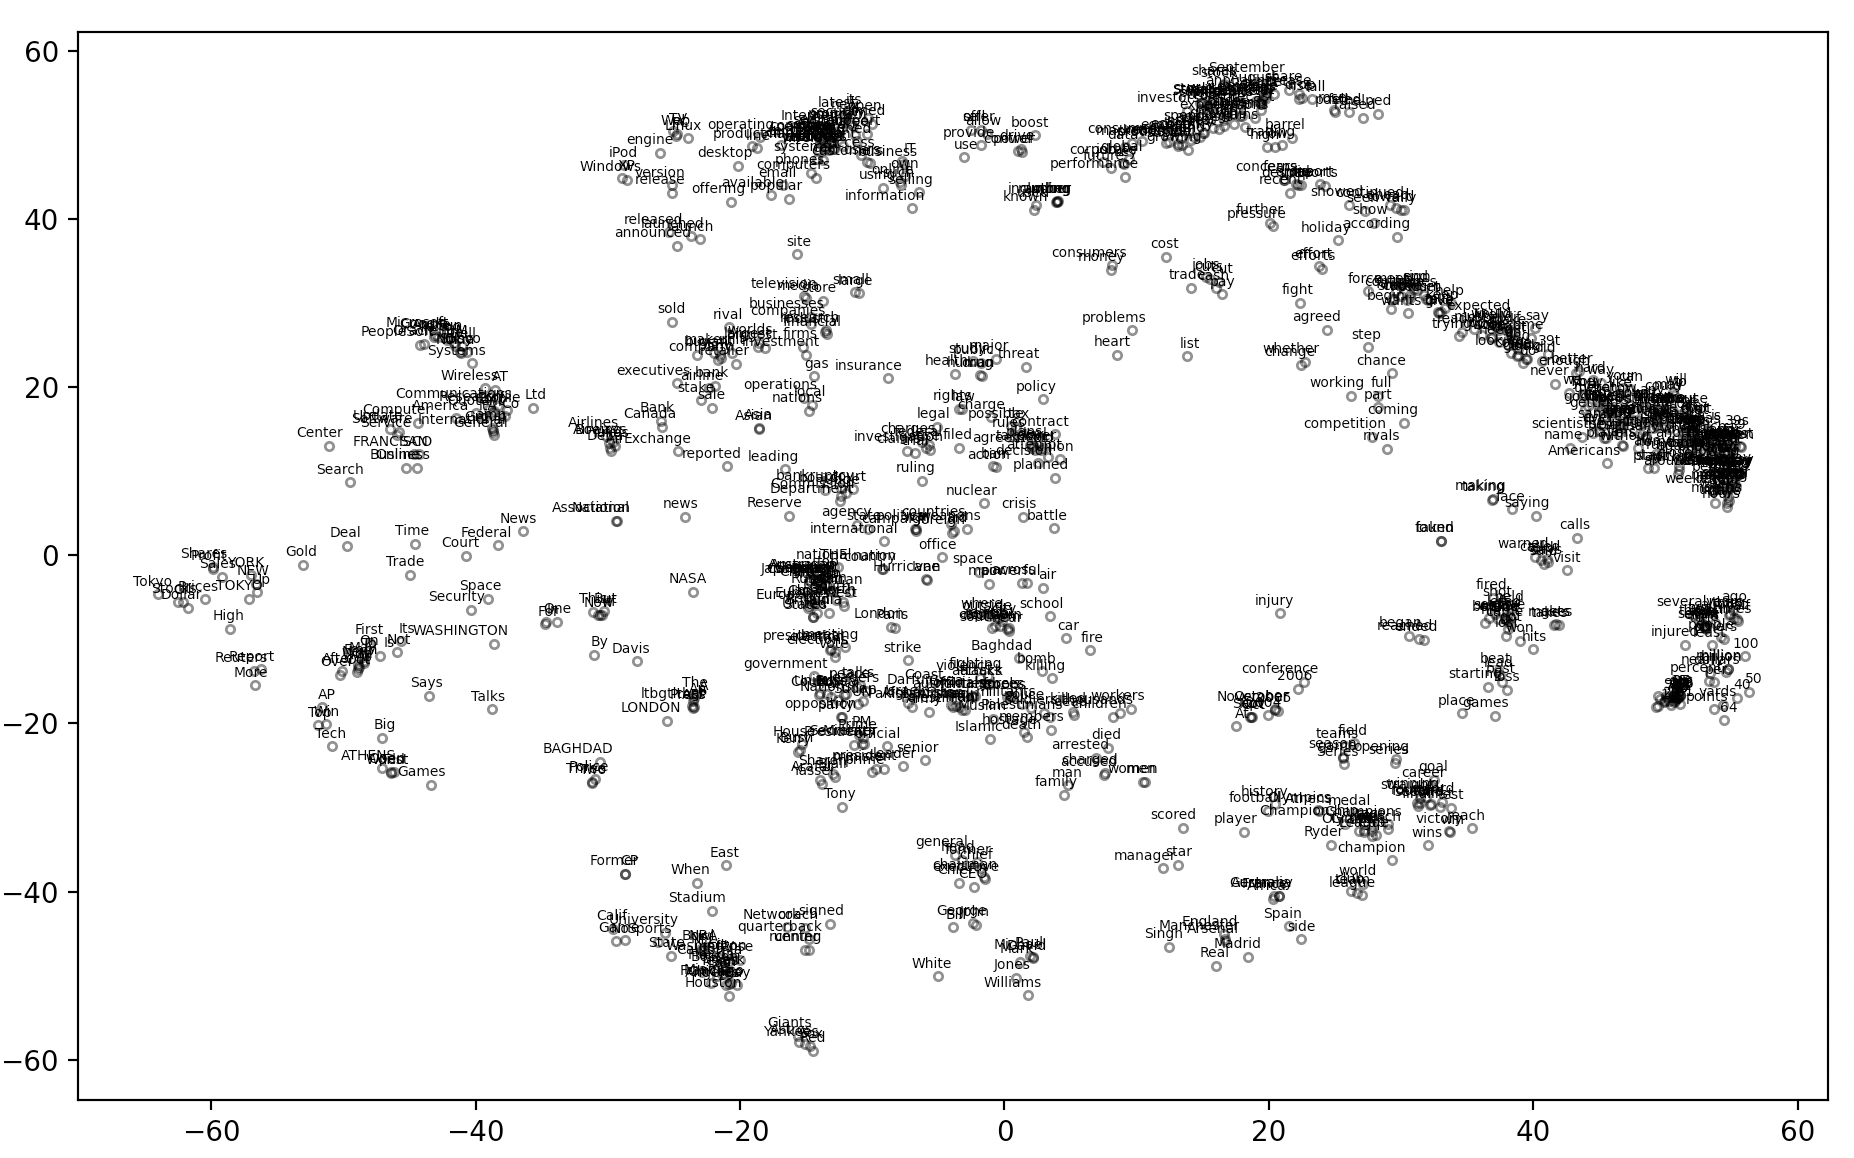
\includegraphics[scale=0.5]{whole_plot.png} \par
    \caption{Whole plot}
    \label{fig:q2-overview}
\end{figure}


\begin{figure}[H]
    \centering
    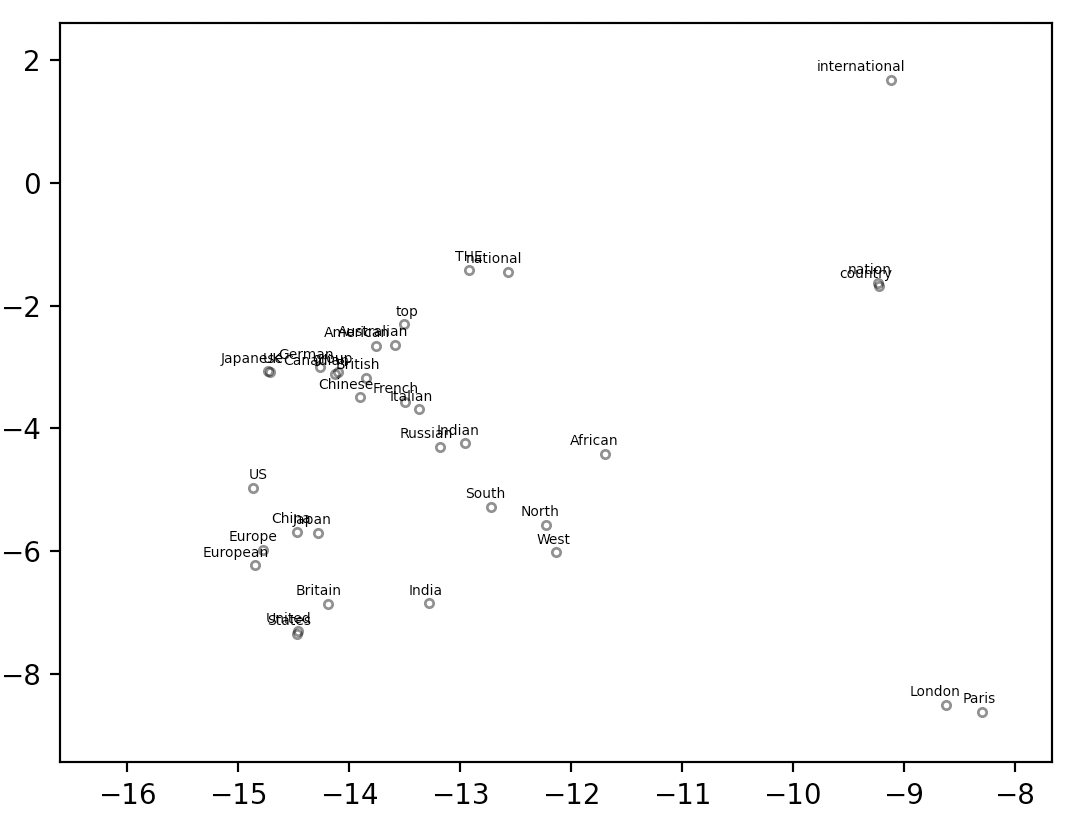
\includegraphics[scale=0.6]{country.png} \par
    \caption{Country cluster}
    \label{fig:q2-country-cluster}
\end{figure}


\begin{figure}[H]
    \centering
    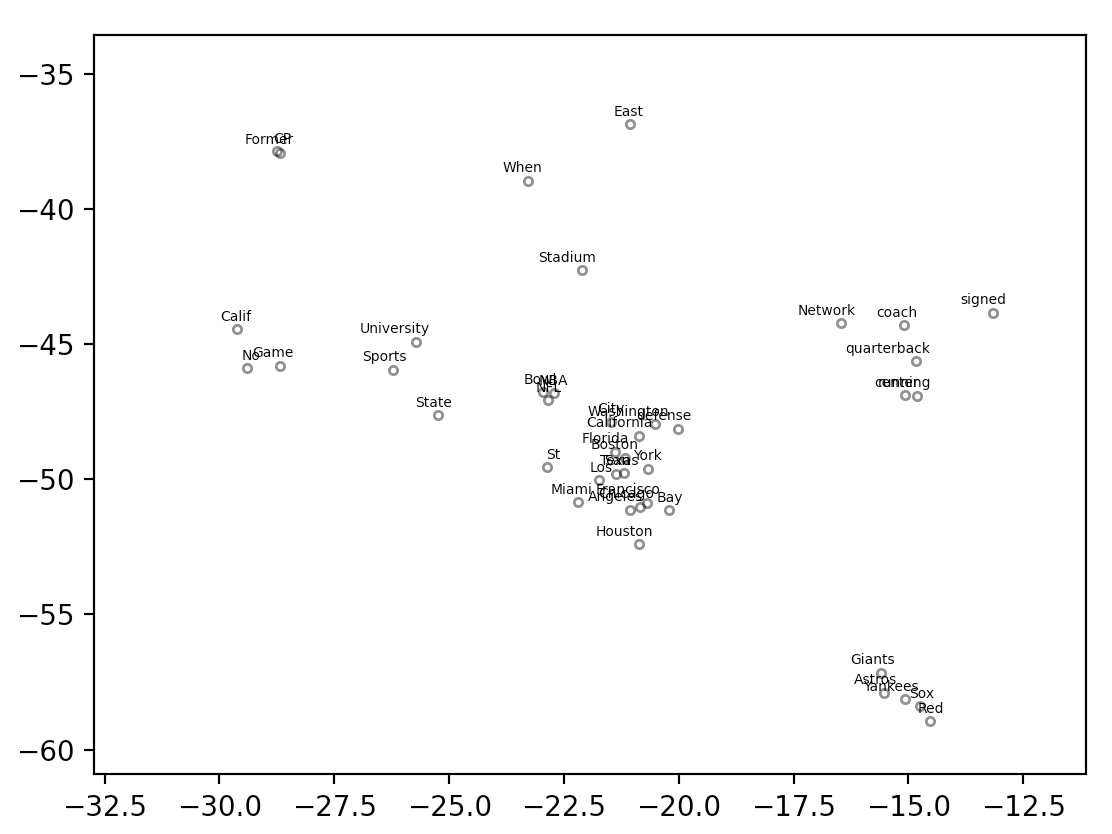
\includegraphics[scale=0.6]{american_football.png} \par
    \caption{American football cluster}
    \label{fig:q2-american-football}
\end{figure}


\begin{figure}[H]
    \centering
    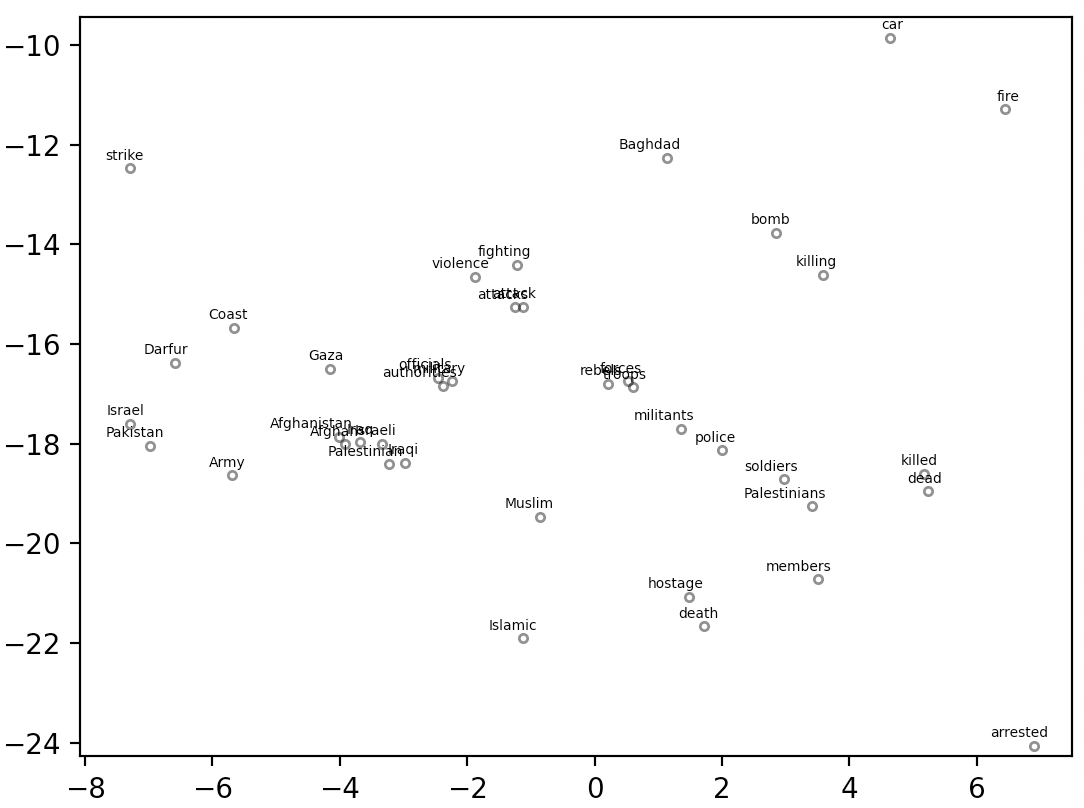
\includegraphics[scale=0.6]{middleeast_war.png} \par
    \caption{Middle East war cluster}
    \label{fig:q2-middle-east}
\end{figure}

%==============================================================================%
\newpage
\begin{task}{3.1}
Derive the gradient of the objective $J_B$ with respect to the model parameters $w_i, \widetilde{w}_j, b_i, \widetilde{b}_j$. That is, write the expression for $\triangledown_{w_i}J, \triangledown_{\widetilde{w}_j}J, \triangledown_{b_i}J, \triangledown_{\widetilde{b}_j}J$. Note that parameters corresponding to words not in B will have zero gradient.
\end{task}
$$\nabla_{w_i}J = \sum_{(i_m,j_m) \in B} 2 f(C_{i_mj_m})(w_{i_m}^T\widetilde{w}_{j_m} + b_{i_m} + \widetilde{b}_{j_m} - logC_{i_mj_m})\widetilde{w}_{j_m}$$

$$\nabla_{\widetilde{w}_j}J = \sum_{(i_m,j_m) \in B} 2 f(C_{i_mj_m})(w_{i_m}^T\widetilde{w}_{j_m} + b_{i_m} + \widetilde{b}_{j_m} - logC_{i_mj_m})w_{i_m}$$

$$\nabla_{b_i}J = \sum_{(i_m,j_m) \in B} 2 f(C_{i_mj_m})(w_{i_m}^T\widetilde{w}_{j_m} + b_{i_m} + \widetilde{b}_{j_m} - logC_{i_mj_m})$$

$$\nabla_{\widetilde{b}_j}J = \sum_{(i_m,j_m) \in B} 2 f(C_{i_mj_m})(w_{i_m}^T\widetilde{w}_{j_m} + b_{i_m} + \widetilde{b}_{j_m} - logC_{i_mj_m})$$

%==============================================================================%
\begin{task}{3.2} 
Implement the gradient computation for a batch in the corresponding Task 3.2 section of build\_glove\_vectors.py.
\end{task}

\small{
\begin{lstlisting}[language=Python]
    c_biases_grad = w_biases_grad = np.multiply(np.multiply(fval, 2), error)
    wordvecs_grad = np.multiply(wordbiases_grad, c_batch)
    contextvecs_grad = np.multiply(contextbiases_grad, w_batch)
\end{lstlisting}
}

%==============================================================================%
\newpage
\begin{task}{3.3} 
Run build\_glove\_vectors.py to learn GloVe vectors and visualize them with TSNE! In your write-up, describe how the loss behaved during training (how stably it decreased, what it converged to, etc). Also include the TSNE plot. If everything has been done correctly, you should observe similar clustering behavior as in Task 2.3.
\end{task}

The model was trained with combinations of various values of batch size, dimensionality, and learning rate in 40 epochs. As can be seen in Figure \ref{fig:q3-hyperparameters-b1024} and \ref{fig:q3-hyperparameters-b2048}, the average loss monotonically decreased after each epoch for all of the combinations. The losses droped significantly at the first 2 epochs, then gradually decreased until plateauing at around 0.03. Training with batch size of 2048, dimensionality of 64, and learning rate of 0.08 yielded the best performance, reaching the loss of approximately 0.028 after 40 epochs.

\begin{figure}[H]
    \centering
    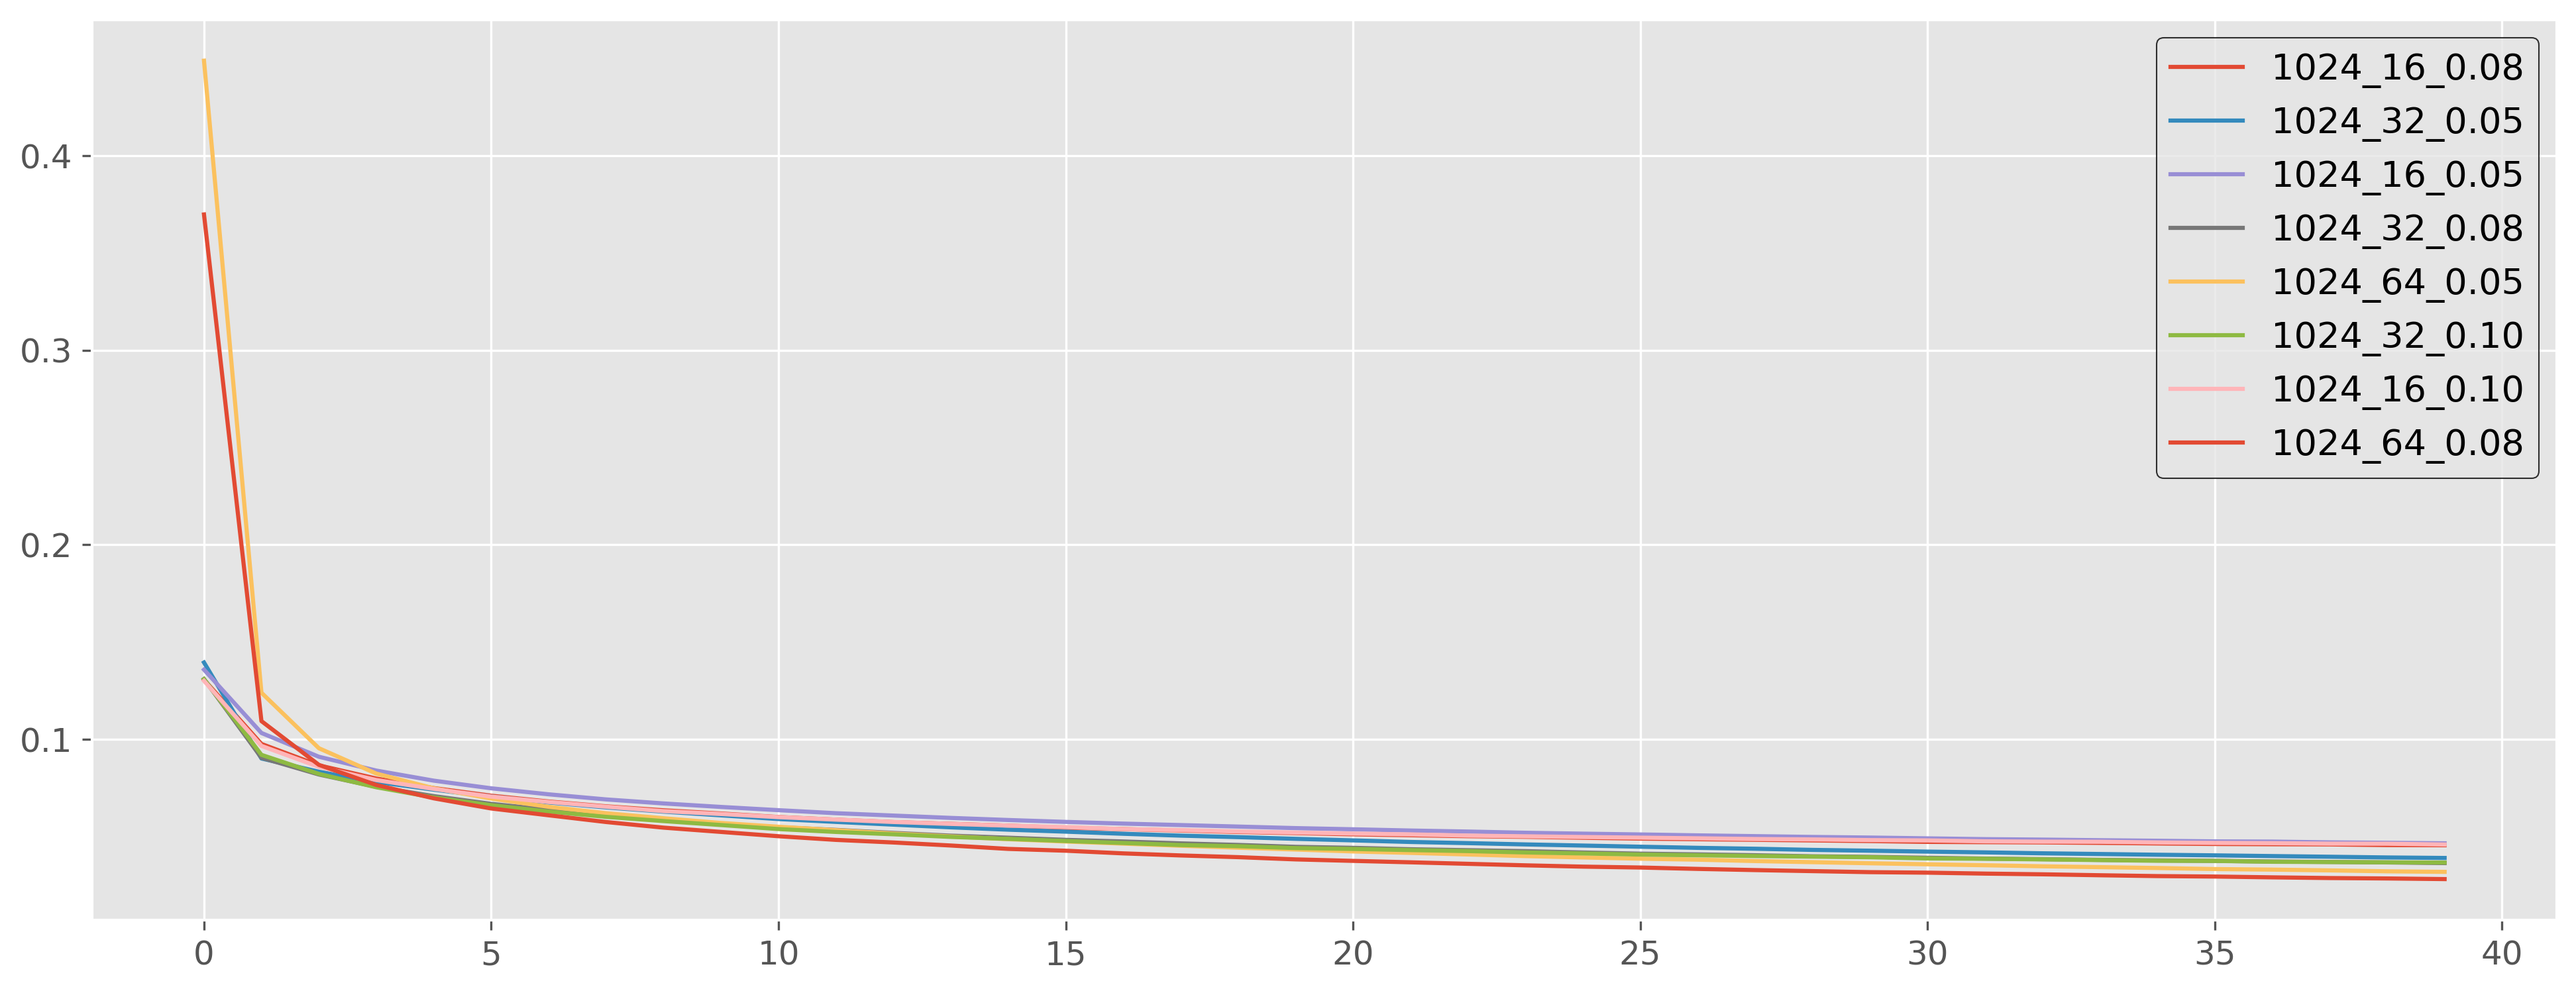
\includegraphics[scale=0.5]{glove_tuning_1024.png} \par
    \caption{Hyperparameters tuning with batch size of 1024}
    \label{fig:q3-hyperparameters-b1024}
\end{figure}

\begin{figure}[H]
    \centering
    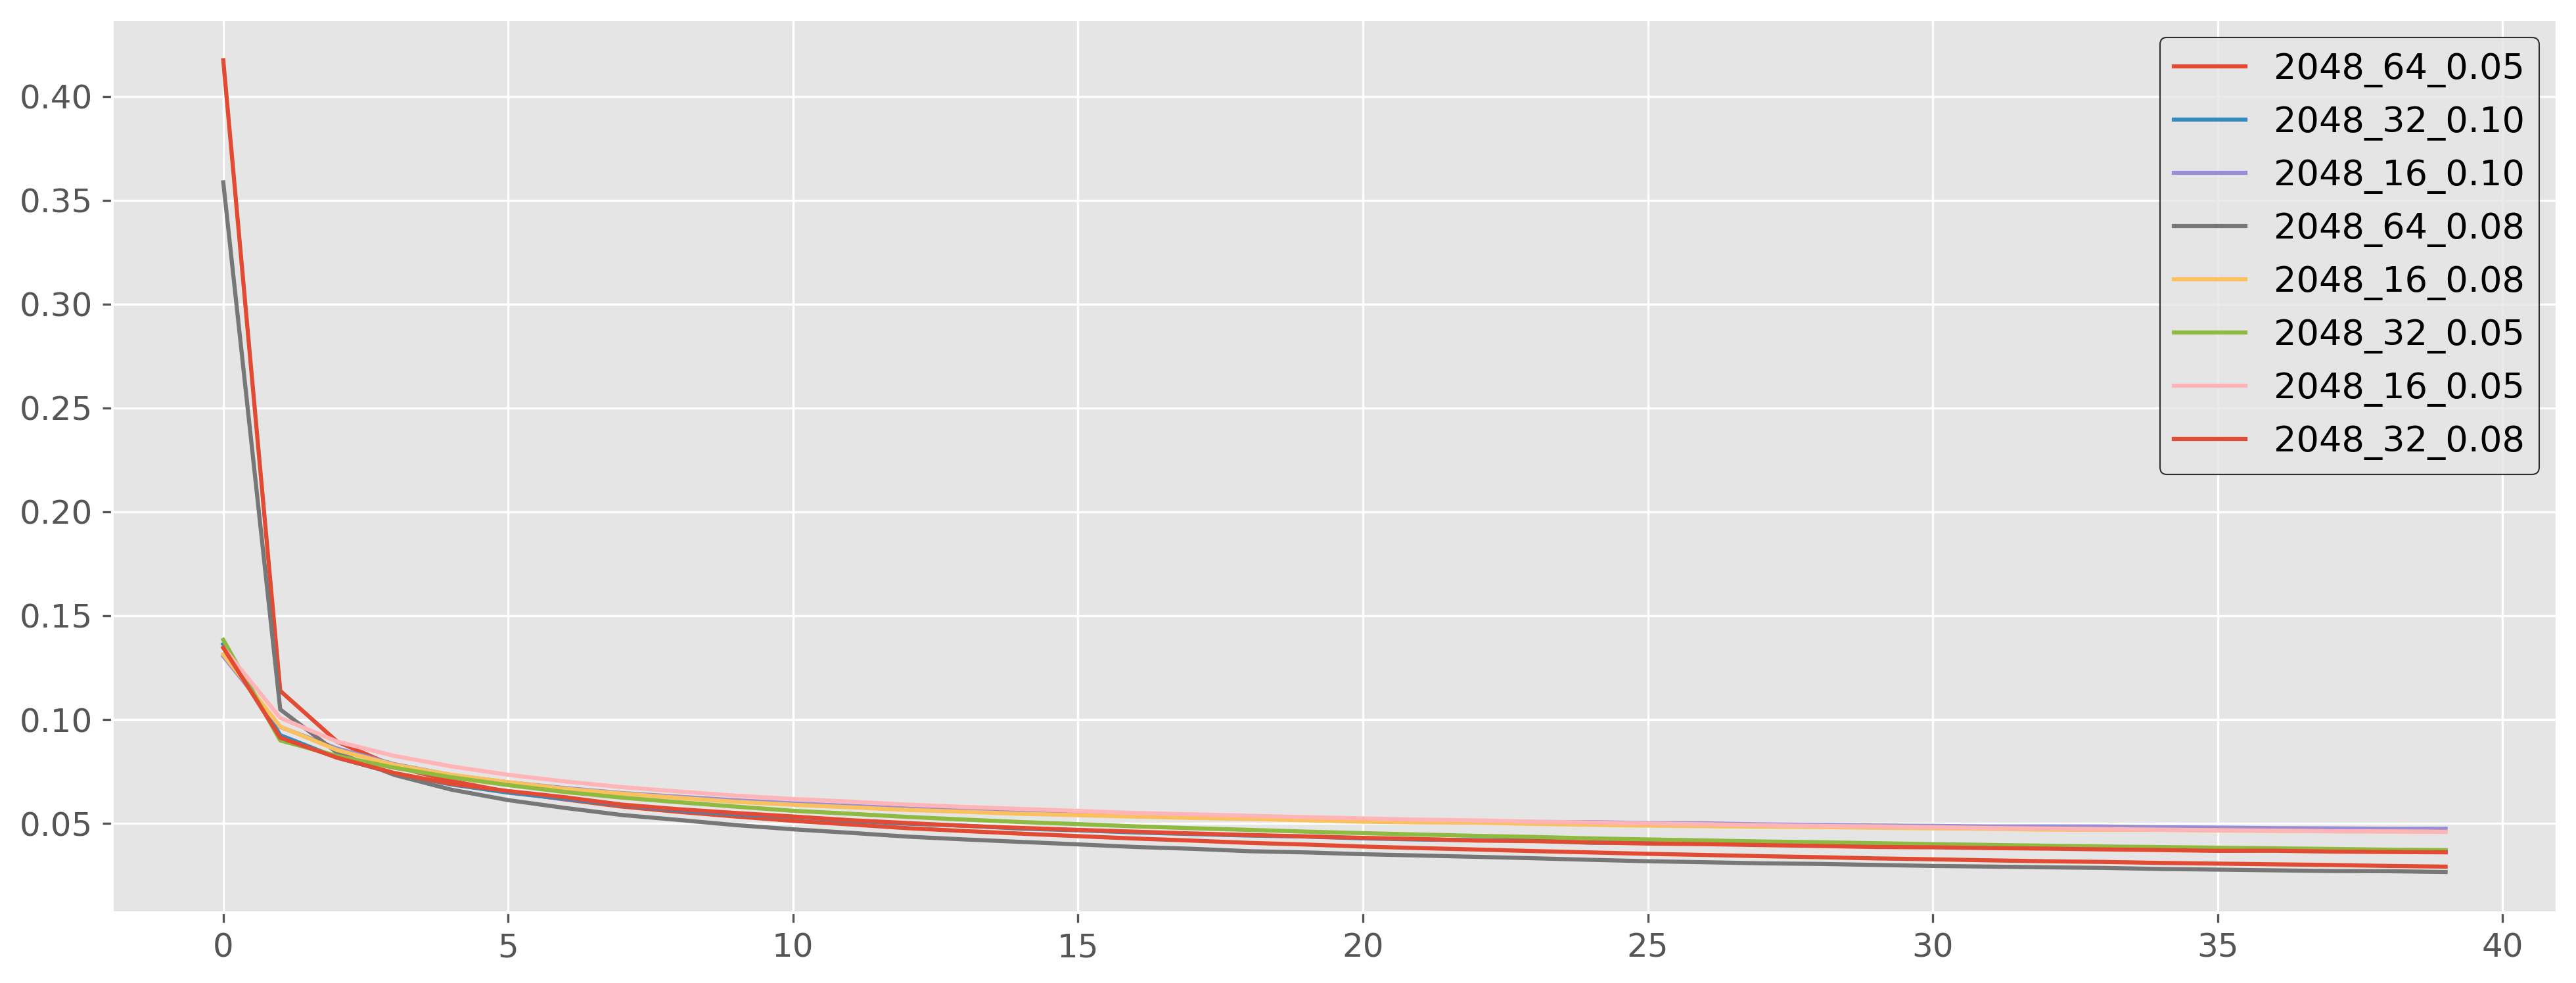
\includegraphics[scale=0.5]{glove_tuning_2048.png} \par
    \caption{Hyperparameters tuning with batch size of 2048}
    \label{fig:q3-hyperparameters-b2048}
\end{figure}

\newpage

Figure \ref{fig:q3-tsne-overview} shows TSNE plot of the best model. Similar clusters to those in task 2.4 can be observed in this plot. In particular, \ref{fig:q3-tsne-location} shows a cluster of locations and \ref{fig:q3-tsne-quantity} shows a cluster of quantities.

\begin{figure}[H]
    \centering
    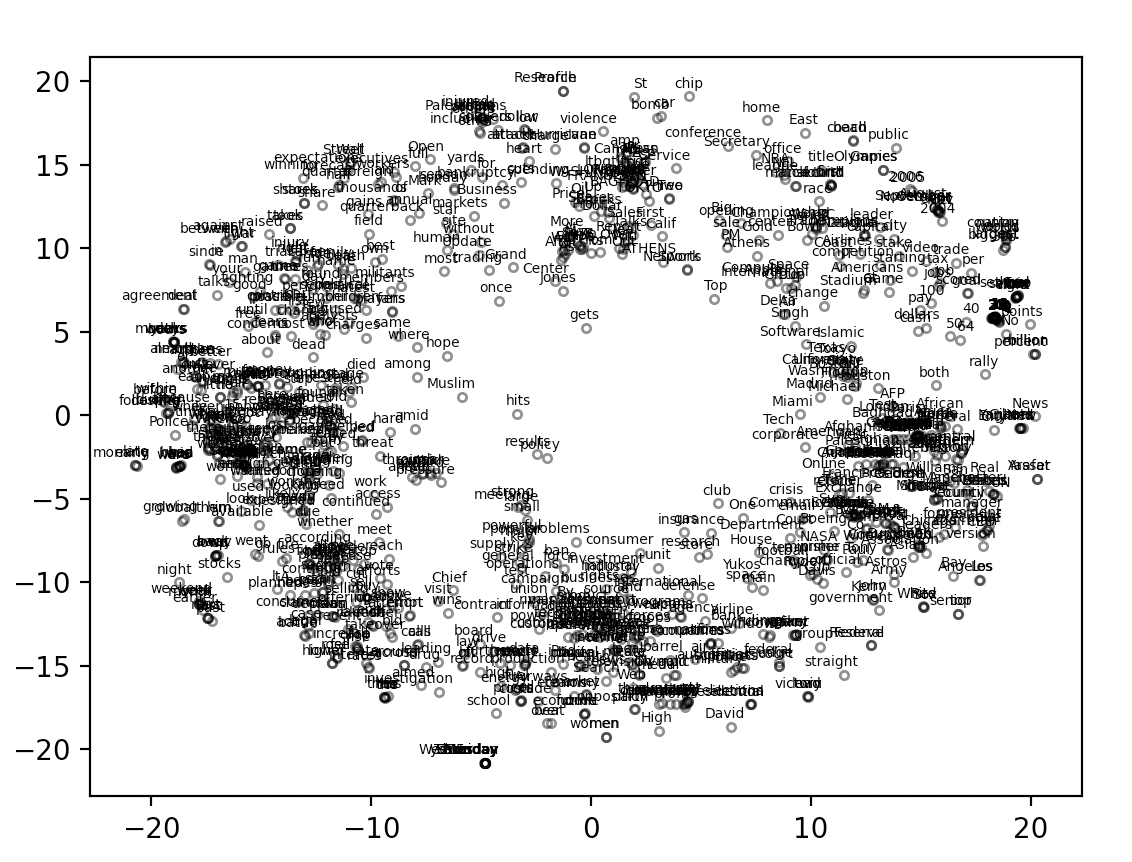
\includegraphics[scale=0.5]{glove_tsne_birdview.png} \par
    \caption{GloVe TSNE bird's-eye view}
    \label{fig:q3-tsne-overview}
\end{figure}

\begin{figure}[H]
    \centering
    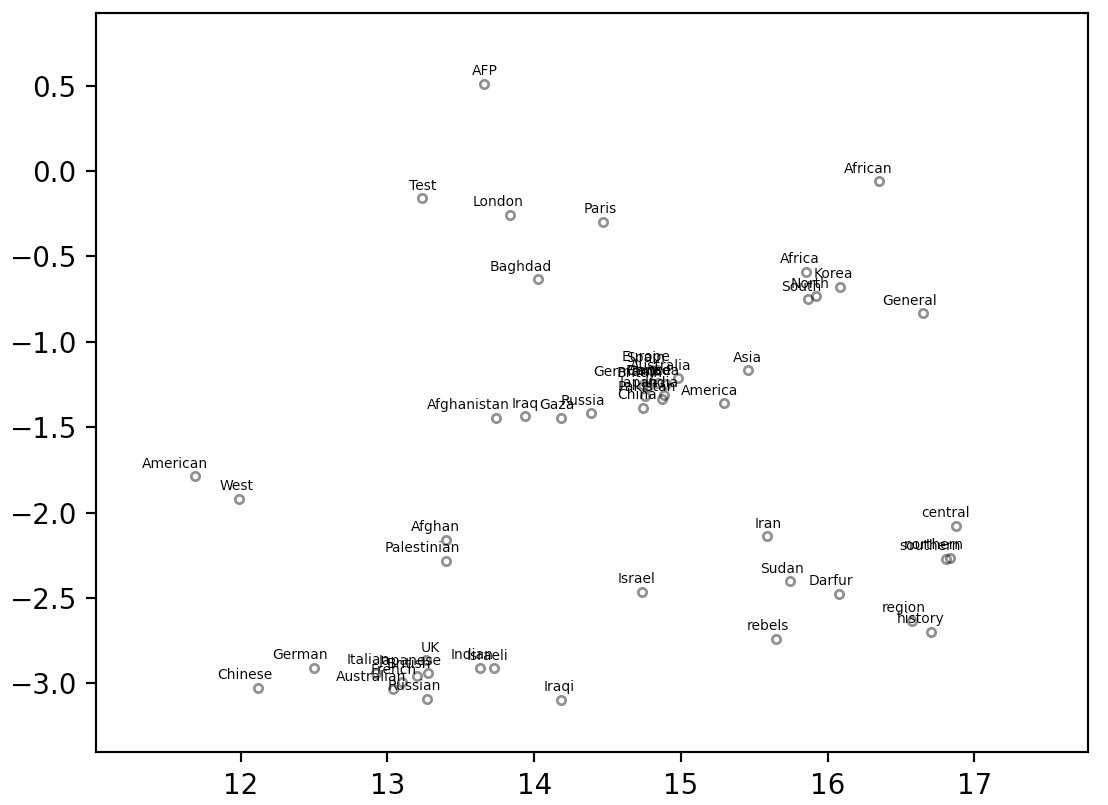
\includegraphics[scale=0.5]{glove_tsne_location_cluster.png} \par
    \caption{GloVe TSNE location cluster}
    \label{fig:q3-tsne-location}
\end{figure}

\begin{figure}[H]
    \centering
    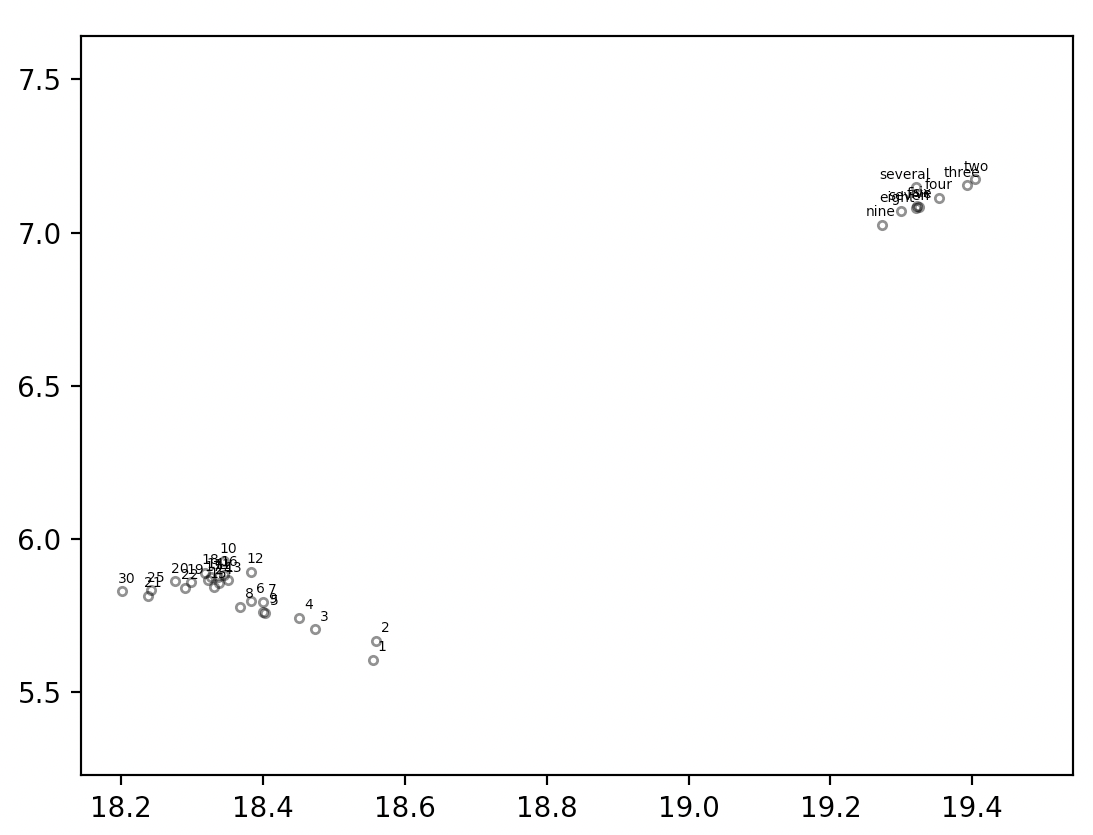
\includegraphics[scale=0.5]{glove_tsne_quantity_cluster.png} \par
    \caption{GloVe TSNE quantity cluster}
    \label{fig:q3-tsne-quantity}
\end{figure}
%==============================================================================%
\newpage
\begin{task}{4.1} 
Use the most\_similar function to find three additional analogies that work. In your response, provide the analogies in the compact a:b::c:? form, the model's list of outputs, and why you consider this output to satisfy the analogy.
\end{task}
Table \ref{table:q4-reasonable-analogies} shows three reasonable analogies. First, "Messi : Argentina :: Neymar : ?" returned Brazil, which is indeed the country which the famous soccer player Neymar comes from as Messi comes from Argentina. Second, football is used in the United Kingdom as soccer is used in Canada and the US. Finally, Paris is the capical of France as Beijing is that of China.

\begin{table}[H]
    \caption{reasonable analogies, Messi:Argentina::Neymar:?, football:uk::soccer:?, China:Beijing::France:?, in order from left to right}
    \label{table:q4-reasonable-analogies}
\hspace{50pt}
\begin{minipage}[c]{0.25\linewidth}%
    \scalebox{0.9}{
    \begin{tabular}{|c|c|}
        \hline
        \textbf{word} & \textbf{cosine}  \\
        \hline
        Brazil & 0.622\\
        \hline
        Uruguay & 0.581\\
        \hline
        Chile & 0.561\\
        \hline
        Ecuador & 0.56\\
        \hline
        Argentine & 0.555\\
        \hline
        Argentinean & 0.535\\
        \hline
        Paraguay & 0.525\\
        \hline
        Peru & 0.521\\
        \hline
        Argentinian & 0.505\\
        \hline
        striker\_Neymar & 0.503\\
        \hline
\end{tabular}}
 %\captionof{figure}{29 most similar\newline words to "good"}
\end{minipage}
\hspace{0pt}%
\begin{minipage}[c]{0.25\linewidth}%
    \scalebox{0.9}{
    \begin{tabular}{|c|c|}
        \hline
        \textbf{word} & \textbf{cosine}  \\
        \hline
        canada &  0.585 \\
        \hline
        usa &  0.585 \\
        \hline
        australia &  0.525 \\
        \hline
        india &  0.511 \\
        \hline
        germany &  0.502 \\
        \hline
        malaysia &  0.501 \\
        \hline
        amsterdam &  0.5 \\
        \hline
        denmark &  0.496 \\
        \hline
        thailand &  0.488 \\
        \hline
        bbc &  0.483 \\
        \hline
\end{tabular}}
 %\captionof{figure}{29 most similar\newline words to "good"}
\end{minipage}
\hspace{-18pt}%
\begin{minipage}[c]{0.25\linewidth}%
    \scalebox{0.9}{
    \begin{tabular}{|c|c|}
       \hline
       \textbf{word} & \textbf{cosine}  \\
       \hline
        Paris &  0.721 \\
        \hline
        French &  0.624 \\
        \hline
        Colombes &  0.609 \\
        \hline
        Marseille &  0.597 \\
        \hline
        Melun &  0.589 \\
        \hline
        Aix\_en\_Provence &  0.578 \\
        \hline
        Issy\_les\_Moulineaux &  0.578 \\
        \hline
        Montpellier &  0.574 \\
        \hline
        Toulouse &  0.571 \\
        \hline
        Nantes &  0.566 \\
        \hline
\end{tabular}}
\end{minipage}
\end{table}

%==============================================================================%
\newpage
\begin{task}{4.2} 
Use the most\_similar function to find three analogies that did not work. In your response to this question, provide the analogies in the compact a:b::c:? form, the model's list of outputs, and why you consider this output to not satisfy the analogy.
\end{task}

Table \ref{table:q4-unreasonable-analogies} shows three reasonable analogies. First, although the analogy works out for China and France as shown in Table \ref{table:q4-reasonable-analogies}, it does not work for China and the US. Second, the model cannot relate Beyonce to the US as Adele is a famous female singer from England. Lastly, the model cannot relate CIA to the US as FIS, the Foreign Intelligence Service of the Russian Federation, is to Russia.

\begin{table}[H]
    \caption{unreasonable analogies, China:Beijing::United\_States:?, Adele:England::Beyonce:?, FIS:Russia::CIA:?, in order from left to right}
    \label{table:q4-unreasonable-analogies}
\hspace{0pt}
\begin{minipage}[c]{0.25\linewidth}%
    \scalebox{0.9}{
    \begin{tabular}{|c|c|}
        \hline
        \textbf{word} & \textbf{cosine}  \\
        \hline
        Unites\_States &  0.58 \\
        \hline
        U.S. &  0.569 \\
        \hline
        United\_Sates &  0.539 \\
        \hline
        Untied\_States &  0.532 \\
        \hline
        theUnited\_States &  0.488 \\
        \hline
        Washington\_DC &  0.477 \\
        \hline
        Washington &  0.465 \\
        \hline
        UnitedStates &  0.453 \\
        \hline
        Great\_Britain &  0.444 \\
        \hline
        Athens\_Greece &  0.439 \\
        \hline
\end{tabular}}
 %\captionof{figure}{29 most similar\newline words to "good"}
\end{minipage}
\hspace{5pt}%
\begin{minipage}[c]{0.25\linewidth}%
    \scalebox{0.9}{
    \begin{tabular}{|c|c|}
        \hline
        \textbf{word} & \textbf{cosine}  \\
        \hline
        stock\_symbol\_BNK &  0.467 \\ 
        \hline
        Freddie\_Flintoff &  0.458 \\ 
        \hline
        ticker\_symbol\_BNK &  0.455 \\ 
        \hline
        DAILY\_STAR\_Fabio\_Capello &  0.446 \\ 
        \hline
        Wayne\_Rooney &  0.446 \\ 
        \hline
        David\_Beckham &  0.444 \\ 
        \hline
        NatWest\_Challenge &  0.437 \\ 
        \hline
        Beyoncé &  0.434 \\ 
        \hline
        Frank\_Lampard &  0.429 \\ 
        \hline
        midfielder\_Frank\_Lampard &  0.427 \\
        \hline
\end{tabular}}
\end{minipage}
\hspace{60pt}%
\begin{minipage}[c]{0.25\linewidth}%
    \scalebox{0.9}{
    \begin{tabular}{|c|c|}
       \hline
       \textbf{word} & \textbf{cosine}  \\
       \hline 
        Kremlin &  0.506 \\ 
        \hline 
        former\_Soviet\_republics &  0.494 \\ 
        \hline 
        Moscow &  0.482 \\ 
        \hline 
        Soviet &  0.474 \\ 
        \hline 
        former\_Soviet\_Republics &  0.473 \\ 
        \hline 
        CIA\_operatives &  0.47 \\ 
        \hline 
        Russian &  0.467 \\ 
        \hline 
        Soviet\_Union &  0.466 \\ 
        \hline 
        Ukraine &  0.465 \\ 
        \hline 
        spy &  0.46 \\
        \hline
\end{tabular}}
\end{minipage}
\end{table}

%==============================================================================%
\newpage
\begin{task}{4.3} 
Use the most\_similar function to find two additional cases of bias based on gender, politics, religion, ethnicity, or nationality. In your response, provide the analogies in the compact a:b::c:? form, the model's list of outputs for both a:b::c:? and c:b::a:?, and why you consider this output to be biased based on the model's two responses.
\end{task}

Table \ref{table:q4-gender_bias} demonstrates gender bias in word2vec. In particular, when the model was asked boy:soccer::girl:?, volleyball and softball are the most similar instead of soccer. On the other hand, girl:soccer::boy:? returned soccer as the most similar word. This implies that boys are more likely to play soccer than girls.

\begin{table}[H]
    \caption{bias based on gender in word2vec. The left table shows the most similar to boy:soccer::girl:? and the right table shows the most similar words to girl:soccer::boy:?}
    \label{table:q4-gender_bias}
\hspace{120pt}
\begin{minipage}[c]{0.25\linewidth}%
    \scalebox{0.9}{
    \begin{tabular}{|c|c|}
        \hline
        \textbf{word} & \textbf{cosine}  \\
        \hline
        volleyball &  0.694 \\ 
        \hline
        softball &  0.668 \\ 
        \hline
        Soccer &  0.649 \\ 
        \hline
        basketball &  0.632 \\ 
        \hline
        lacrosse &  0.618 \\ 
        \hline
        water\_polo &  0.596 \\ 
        \hline
        football &  0.596 \\ 
        \hline
        Volleyball &  0.589 \\ 
        \hline
        tennis &  0.585 \\ 
        \hline
        hockey &  0.564 \\
        \hline
\end{tabular}}
\end{minipage}
\hspace{5pt}%
\begin{minipage}[c]{0.25\linewidth}%
    \scalebox{0.9}{
    \begin{tabular}{|c|c|}
        \hline
        \textbf{word} & \textbf{cosine}  \\
        \hline
        Soccer &  0.692 \\ 
        \hline
        football &  0.692 \\ 
        \hline
        basketball &  0.566 \\ 
        \hline
        fooball &  0.545 \\ 
        \hline
        sports &  0.542 \\ 
        \hline
        baseball &  0.542 \\ 
        \hline
        futbol &  0.542 \\ 
        \hline
        hockey &  0.54 \\ 
        \hline
        SOCCER &  0.532 \\ 
        \hline
        Futsal &  0.518 \\
        \hline
\end{tabular}}
\end{minipage}
\end{table}

Researchers found that there are association between names and races. For example, Gabe has 86\% probability of being a White person's name, whereas 70\% percent of people named Miguel are Hispanic \cite{BiasInEmbedding}. More interestingly, word2vec shows that Miguel is much more similar to smugglers than Gabe is. Particularly, as shown by Table \ref{table:q4-race_bias}, Miguel:smuggler::Gabe:? returned smugglers with 0.486 cosine similarity, while Gabe:smuggler::Miguel:? produced smugglers with much higher similarity, at 0.596. This implies that a Hispanic is more associated with smugglers than a White person.

\begin{table}[H]
    \caption[justification=centering]{bias based on race in word2vec. The left table shows the most similar to Miguel:smuggler::Gabe:? and the right table shows the most similar words to Gabe:smuggler::Miguel:?}
    \label{table:q4-race_bias}
\hspace{90pt}
\begin{minipage}[c]{0.25\linewidth}%
    \scalebox{0.9}{
    \begin{tabular}{|c|c|}
        \hline
        \textbf{word} & \textbf{cosine}  \\
        \hline
        smugglers &  0.486 \\ 
        \hline
        smuggling &  0.449 \\ 
        \hline
        Smugglers &  0.406 \\ 
        \hline
        smuggled &  0.397 \\ 
        \hline
        Rabiyah &  0.387 \\ 
        \hline
        trafficker &  0.386 \\ 
        \hline
        smuggle &  0.385 \\ 
        \hline
        drug\_smuggler &  0.378 \\ 
        \hline
        Zach &  0.375 \\ 
        \hline
        informant &  0.373 \\
        \hline
\end{tabular}}
\end{minipage}
\hspace{5pt}%
\begin{minipage}[c]{0.25\linewidth}%
    \scalebox{0.9}{
    \begin{tabular}{|c|c|}
        \hline
        \textbf{word} & \textbf{cosine}  \\
        \hline
        smugglers &  0.596 \\ 
        \hline
        migrant\_smuggler &  0.542 \\ 
        \hline
        trafficker &  0.54 \\ 
        \hline
        smuggling &  0.529 \\ 
        \hline
        traffickers &  0.507 \\ 
        \hline
        drug\_trafficker &  0.505 \\ 
        \hline
        Colombian\_traffickers &  0.504 \\ 
        \hline
        Juárez\_Cartel &  0.501 \\ 
        \hline
        immigrant\_smuggler &  0.494 \\ 
        \hline
        border\_crosser &  0.483 \\
        \hline
\end{tabular}}
\end{minipage}
\end{table}
%==============================================================================%
\begin{task}{4.4} 
Why might these biases exist in word2vec and what are some potential consequences that might result if word2vec were used in a live system?
\end{task}

Word2vec contains biases because it captures hidden stereotypes present in the society. In case of "word2vec-google-news-300", it is professional journalists' negative beliefs towards gender and race that were quantified by the model \cite{DebiasingWordEmbeddings}. Word embeddings have become the defacto standard method to represent text data in many NLP tasks. Therefore, latent biases contained in these models could be learned by NLP models, which might pose a risk of reinforcing stereotypes in society.

\bibliographystyle{alpha}
\bibliography{mybib}
\end{document}
